% ===================================================================
%                   Presentación con Latex Beamer
% ===================================================================
\documentclass[9pt,xcolor=svgnames]{beamer}
%\documentclass[handout,xcolor=svgnames]{beamer} %Version imprimible
% -------------------------------------------------------------------
% Paquetes personalizados
\usepackage{../paquetes}
\usepackage{../colores}
\usepackage{../info}
\usepackage{../modo}
% -------------------------------------------------------------------

% Comienza el documento
\begin{document}
% Tikz -> Imágenes
\tikzstyle{every picture}+=[remember picture]
% Entorno matemático
\everymath{\displaystyle}
% -------------------------------------------------------------------
\subtitle{El retorno del proyecto}
\date{Mayo 2009}
% -------------------------------------------------------------------
% Fondo blanco: primera página
% ------------------------------------------------------------------

\beamersetaveragebackground{white}

\begin{frame}
 \thispagestyle{empty}
 \begin{figure}[t]
  \centering
  
\includegraphics[scale=0.4]{./Imagenes/logo_cachimba.pdf}

\noindent \Huge Presenta...
\end{figure}
\end{frame}


\begin{frame}
 \thispagestyle{empty}
 
 \animate<2-3> 
 \begin{figure}[t]
  \centering
  \includegraphics<1>[scale=0.7]{../Imagenes/logo_1.pdf}
  \includegraphics<2>[scale=0.7]{../Imagenes/logo_2.pdf}
  \includegraphics<3>[scale=0.7]{../Imagenes/logo_3.pdf}
  \includegraphics<4>[scale=0.7]{../Imagenes/logo_4.pdf}
 \end{figure}
\end{frame}


% -------------------------------------------------------------------
% Fondo para el resto del documento
\setbeamertemplate{background}{

\includegraphics[width=\paperwidth,height=\paperheight]
{../Imagenes/fondo.pdf}
}
% -------------------------------------------------------------------


% Continuación:
% Transparencia de Inicio -> Título
\begin{frame}
 \titlepage
\end{frame}

\normalsize

% Transparencia de índice
\begin{frame}{Índice} 
 \transdissolve
 \tableofcontents
\end{frame}
  
  
 \section{Estado del proyecto}
 
  \subsection{Actualización de la planificación}
  
  \begin{frame}{Diagrama de Gannt}
   
%   \begin{figure}[t]
%    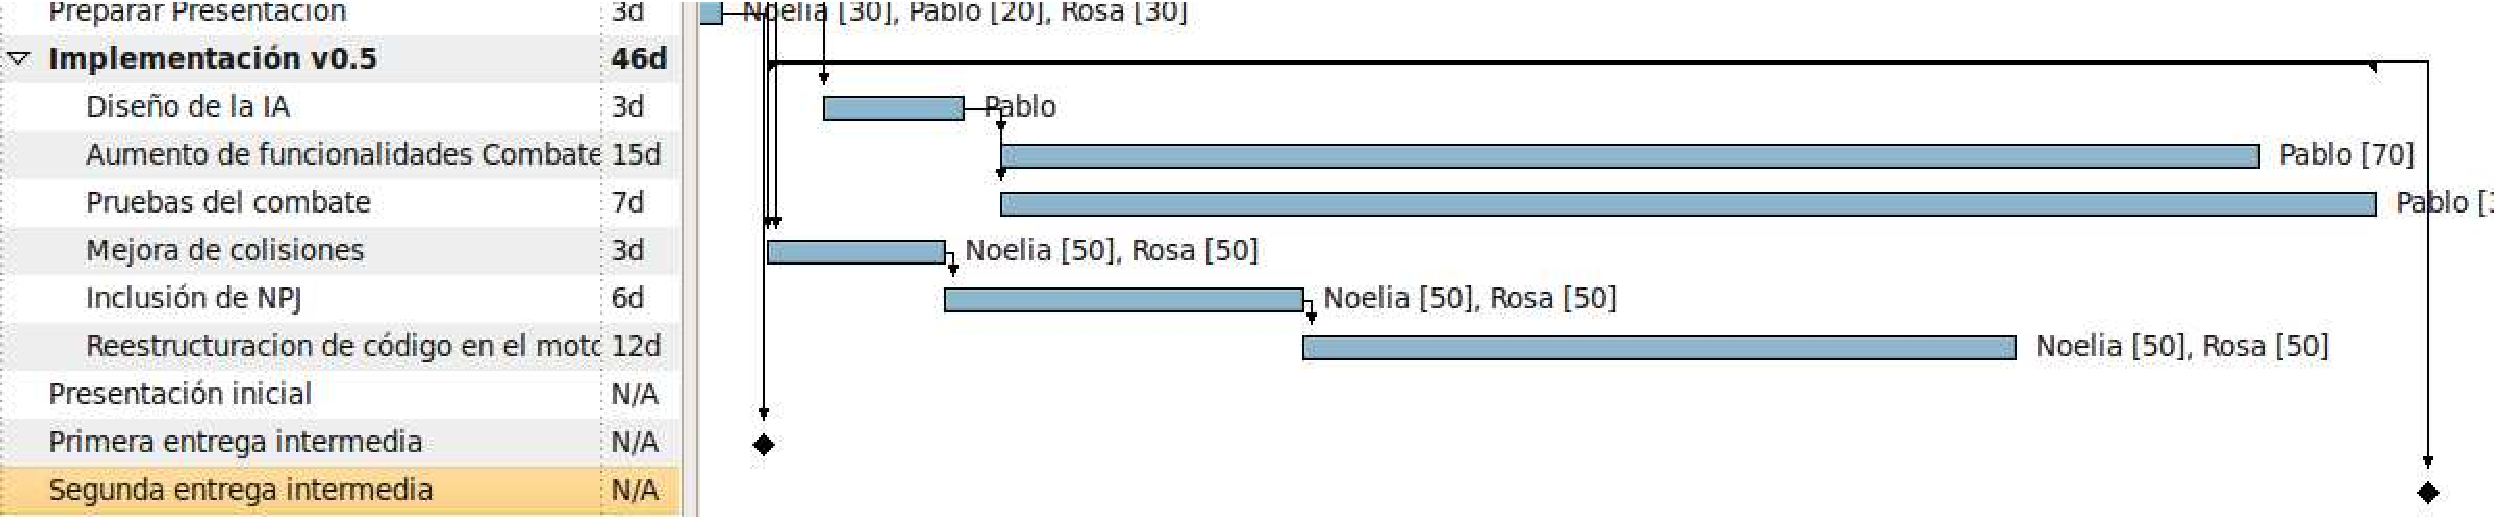
\includegraphics[scale=0.27]{./Imagenes/gannt.pdf}
%   \end{figure}
   
  \end{frame}
  
  
  \begin{frame}{Asignación de Recursos}
   
   Seguimos centrándonos en la implementación:
   
    
  \end{frame}
   
   
   
   \subsection{Modificaciones sufridas por el proyecto}
   
   \begin{frame}{Modificaciones y justificaciones}
    
    ¿?
    
    
   \end{frame}
   
   
 \section{Presentación Previa del producto}
 
   \subsection{Producto actual}

   \begin{frame}{Captura de pantalla: Motor de combate}
    
   \end{frame}


   \begin{frame}{Captura de pantalla: Motor gráfico}
    
   \end{frame}



 \section{Calidad de la implementación}
 
  \subsection{Calidad del codigo}
  
  \begin{frame}{Programación Orientada a Objetos + SDL}   
   
   
   \textsc{Nota.} La unión entre los dos motores aún no está
   implementada, puesto que no están terminados los motores.

  \end{frame}
  
  
  \subsection{Ejemplos de código}
  
  \begin{frame}{Ejemplo: Clase x}

  \end{frame}
  
  
  \begin{frame}{Ejemplo: Interfaz principal entre clases}

  \end{frame}
    
  


 \section{Conclusión}
 
  \subsection{Solución de problemas}

  \begin{frame}{Problemas y soluciones}
   
  \end{frame}
  
  
 \section{Para terminar}
  
\scriptsize

 \begin{frame}{Esta presentación es libre}
  Copyright 2009 Noelia Sales Montes\\
  Parte del Proyecto NoCKt Metal\\
  \url{http://nocktmetal.forja.rediris.es/}
  
  \vspace*{0.3cm}
  
  Creative Commons Attribution License
  \url{http://creativecommons.org/licenses/by/2.0/}\\
  Creative Commons, 559 Nathan Abbott Way, Stanford, California 94305,
  USA.
  
  \vspace*{0.3cm}
  
  Este trabajo se publica bajo la siguiente licencia:\\
  Creative Commons Attribution License
  \url{http://creativecommons.org/licenses/by/3.0/}
  
  \vspace*{0.3cm}
  
  Usted es libre de:
  \begin{itemize}
   \item copiar, distribuir y comunicar públicamente la obra
   \item hacer obras derivadas
  \end{itemize}
  
  Bajo las condiciones siguientes:
  \begin{itemize}
   \item Reconocimiento. Debe reconocer los créditos de la obra de la
	 manera especificada por el autor o el licenciador (pero no de una
	 manera que sugiera que tiene su apoyo o apoyan el uso que hace de
	 su obra).
   \item Al reutilizar o distribuir la obra, tiene que dejar bien claro los
	 términos de la licencia de esta obra.
   \item Alguna de estas condiciones puede no aplicarse si se obtiene el
	 permiso del titular de los derechos de autor
   \item Nada en esta licencia menoscaba o restringe los derechos morales
	 del autor.
  \end{itemize}
 \end{frame}


  
\end{document}
 
